\documentclass{article}

\usepackage{amssymb, amsmath, bbm}
\usepackage{geometry}
\usepackage{graphicx, float}

\geometry{margin=1.5in}
\setlength{\parindent}{0pt}
\graphicspath{ {./images/} }

\begin{document}
\section{Problem Statement}

We will consider a spatial Poisson process on $\mathbb{R}^2$ with rate $\lambda = 1$, i.e. the number of points in region with area $A$ follows a Poisson distribution with rate $A$. To model increasing larger samples sizes, we look at $[-\frac{t}{2}, \frac{t}{2}]^2$ for increasing larger $t$.

\bigbreak\textbf{Problem.} If we construct the nearest-neighbor graph on the points contained in $[-\frac{t}{2}, \frac{t}{2}]^2$, what is the expected number of edges that cross the $y$-axis?

\bigbreak For $N \sim \textrm{Po}(t^2)$, let $x_1, \hdots, x_N$ be the points in $[-\frac{t}{2}, \frac{t}{2}]^2$ and let $x_{n(i)}$ be $x_i's$ nearest neighbor. Define
$$X_i = \begin{cases}
1 & \textrm{$x_i$ and $x_{n(i)}$ belong to opposite halves, $x_i \neq x_{n(n(i))}$} \\
\frac{1}{2} & \textrm{$x_i$ and $x_{n(i)}$ belong to opposite halves, $x_i = x_{n(n(i))}$} \\
0 & \textrm{otherwise}
\end{cases}$$
Let $T$ be the total number of crossings. Then
$$\mathbb{E}T = \mathbb{E}[\mathbb{E}[T|N]] = \mathbb{E}_N\left[\sum_{i=1}^n \mathbb{E}{X_i}\right] = \sum_{n=0}^\infty n\mathbb{E}X_1 \frac{t^{2n}e^{-t^2}}{n!} = \mathbb{E}X_1 \sum_{n=0}^\infty n\frac{t^{2n}e^{-t^2}}{n!} = t^2\mathbb{E}X_1$$
It remains to find $\mathbb{E}X_1 = P(X_1 = 1) + \frac{1}{2}P(X_1 = \frac{1}{2})$.

\section{Finding $\mathbb{E}X_1$}

\subsection{Finding $P(X_1 = \frac{1}{2})$}

For brevity, define
$$O = \mathbbm{1}(\textrm{$x_1$ and $x_{n(1)}$ belong to opposite halves})$$
$$D = \mathbbm{1}(x_1 = x_{n(n(1))}$$
Then $P(X_1 = 1) = P(O = 1 \cap D = 1)$. We condition on the distance $d$ between $x_1$ and the $y$-axis. Note $d \sim \textrm{Unif}([0, \frac{t}{2}])$.

\begin{equation}
\begin{split}
P(X_1 = 1|d) &= P(O = 1 \cap D = 1 | d) \\
&= P(D = 1 | O = 1,d) P(O = 1 | | d) \\
&= \int_d^\infty P(D = 1 | O = 1, d, r) f(r | O = 1, d) \:dr * P(O = 1 | d),
\end{split}
\end{equation}
where $r = ||x_1 - x_{n(1)}||$ is the distance between $x_1$ and its nearest neighbor.

\subsubsection{$P(D = 1 | O = 1,d,r)$}

Given $O = 1$, $d$, and $r$, we want to find the probability $x_1 = x_{n(n(1))}$. We condition on $r = ||x_1 - x_{n(1)}||$. Consider the following figure depicting the situation.

\begin{figure}[H]
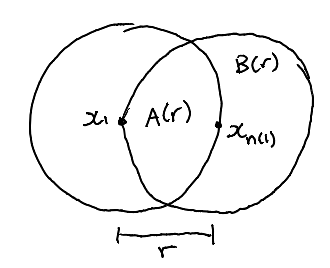
\includegraphics[scale=0.5]{nearest neighbor circles}
\centering
\end{figure}

In order for $x_1 = x_{n(n(1))}$, i.e. $x_1$ is $x_{n(1)}$'s nearest neighbor, there cannot be a point contained in a circle of radius $r$ round $x_{n(1)}$. Since we on condition $r$, we know there does not exist a point in the intersection of the two circles. Hence, $D = 1$ if and only no point lies in the region with area $B(r)$. 
$$B(r) = \pi r^2 - r^2\left(\frac{2\pi}{3} - \frac{\sqrt{3}}{2}\right) = r^2\left(\frac{\pi}{3} + \frac{\sqrt{3}}{2}\right),$$ 
and thus,
$$P(D = 1 | O = 1, d, r) = e^{- r^2\left(\frac{\pi}{3} + \frac{\sqrt{3}}{2}\right)}.$$

\subsubsection{$f(r | O=1,d)$}

According to Bayes' rule,
$$f(r | O=1,d) = \frac{P(O=1 | r,d)f(r | d)}{P(O=1 | d)}.$$
For $f(O=1 | r,d)f(r | d)$ consider the following situation. 

\begin{figure}[H]
\includegraphics[scale=0.5]{d and r known}
\centering
\end{figure}

$x_{n(1)}$ lies somewhere along the circle of radius $r$ centered at $x_1$, which is a distance $d$ away from the $y$-axis. $O = 1$ if and only if $x_{n(1)}$ lies on the arc on the other side of the $y$-axis. Since $x_{n(1)}$ is equally likely to lie anywhere along the circle, this probability is equal to the ratio of the arc length to the circle's circumference, 
$$P(O=1 | r,d) = \frac{2\cos^{-1}\left(\frac{d}{r}\right)r}{2\pi r} = \frac{\cos^{-1}\left(\frac{d}{r}\right)}{\pi}.$$

$r$ is independent of $d$. For all $r_0 \geq 0$, 
$$P(r \leq r_0) = 1 - e^{-\pi r_0^2} \Rightarrow f(r) = 2\pi r e^{-\pi r^2}.$$

For $P(O = 1 | d)$, we condition on $r$ again.
\begin{equation}
\begin{split}
P(O = 1 | d) &= \int_d^\infty P(O = 1 | r,d) f(r | d) \:dr \\
&= \int_d^\infty \frac{\cos^{-1}\left(\frac{d}{r}\right)}{\pi} 2\pi r e^{-\pi r^2} \:dr \\
&= 2\int_d^\infty \cos^{-1}\left(\frac{d}{r}\right) r e^{-\pi r^2} \:dr \\
\end{split}
\end{equation}
Putting it all together,
\begin{equation}
\begin{split}
f(r | O=1,d) &= \frac{P(O=1 | r,d)f(r | d)}{P(O=1 | d)} \\
&= \frac{\frac{\cos^{-1}\left(\frac{d}{r}\right)}{\pi} * 2\pi r e^{-\pi r^2}}{P(O = 1 | d)} \\
&= \frac{\cos^{-1}\left(\frac{d}{r}\right) * 2re^{-\pi r^2}}{P(O = 1 | d)}
\end{split}
\end{equation}

\subsection{Plugging everything in}
\begin{equation}
\begin{split}
P(X_1 = 1|d) &= \int_d^\infty P(D = 1 | O = 1, d, r) f(r | O = 1, d) \:dr * P(O = 1 | d) \\
&= \int_d^\infty P(D = 1 | O = 1, d, r) \frac{P(O=1 | r,d)f(r | d)}{P(O=1 | d)} \:dr * P(O = 1 | d) \\
&= \int_d^\infty P(D = 1 | O = 1, d, r) P(O=1 | r,d)f(r | d) \:dr \\
&= \int_d^\infty e^{- r^2\left(\frac{\pi}{3} + \frac{\sqrt{3}}{2}\right)}\cos^{-1}\left(\frac{d}{r}\right)2re^{-\pi r^2} \:dr
\end{split}
\end{equation}
Since $d \sim \textrm{Unif}([0,\frac{t}{2}])$, it follows that
\begin{equation}
\begin{split}
P(X_1 = 1) &= \int_0^{t/2} P(X_1 = 1 | d) \frac{2}{t} \:dd \\
&= \frac{4}{t} \int_0^{t/2} \int_d^\infty e^{- r^2\left(\frac{\pi}{3} + \frac{\sqrt{3}}{2}\right)}\cos^{-1}\left(\frac{d}{r}\right)re^{-\pi r^2} \:dr \:dd.
\end{split}
\end{equation}

\subsection{Finding $P(X_1 = 1)$}
Note, 
$$P(X_1 = 1) = P(O = 1) - P(X_1 = 1).$$
It remains to solve for $P(O = 1)$. We condition on $r$ and $d$:
\begin{equation}
\begin{split}
P(O = 1) &= \int_0^{t/2} P(O = 1 | d) \frac{2}{t} \:dd \\
&= \int_0^{t/2} \int_d^\infty P(O = 1 | d,r) f(r|d) \:dr \frac{2}{t} \:dd \\
&= \int_0^{t/2} \int_d^\infty \frac{\cos^{-1}\left(\frac{d}{r}\right)}{\pi} 2\pi r e^{-\pi r^2} \:dr \frac{2}{t} \:dd \\
&= \frac{4}{t}\int_0^{t/2} \int_d^\infty \cos^{-1}\left(\frac{d}{r}\right) re^{-\pi r^2} \:dr \:dd
\end{split}
\end{equation}

\section{Solution}
If we define
$$\varphi(t) = \frac{4}{t}\int_0^{t/2} \int_d^\infty \cos^{-1}\left(\frac{d}{r}\right) re^{-\pi r^2} \:dr \:dd$$
$$\theta(t) = \frac{4}{t} \int_0^{t/2} \int_d^\infty e^{- r^2\left(\frac{\pi}{3} + \frac{\sqrt{3}}{2}\right)}\cos^{-1}\left(\frac{d}{r}\right)re^{-\pi r^2} \:dr \:dd$$
then
$$\mathbb{E}X_1 = (\varphi(t) - \theta(t)) - \frac{1}{2}\theta(t) = \varphi(t) - \frac{1}{2}\theta(t).$$
It follows that
$$\mathbb{E}T = t^2\mathbb{E}X_1 = t^2\left[\varphi(t) - \frac{1}{2}\theta(t)\right].$$

\section{Generalizing to Higher Dimension}
If we generalize to higher dimension, the following functions are required:
\begin{itemize}
	\item $s_n(d, r) = $ the ratio of surface areas in an $n$-dimension hypersphere
	\item $f_n(r) = $ the density of distance to the nearest neighbor
	\item $c_n(r) = $ the volume of the crescent created by two overlapping $n$-dimensional hyperspheres
	\end{itemize}
In two dimensions, these functions are
\begin{itemize}
	\item $s_2(d,r) = \frac{2r\cos^{-1}\left(\frac{d}{r}\right)}{2\pi r}$,
	\item $f_2(r) = 2\pi re^{-\pi r^2}$, and
	\item $c_2(r) = -r^2\left(\frac{\pi}{3} + \frac{\sqrt{3}}{2}\right)$.
\end{itemize}
Using these functions,
\begin{itemize}
	\item $\varphi_n(t) = \frac{2}{t} \int_0^{t/2} \int_0^\infty s_n(d,r)f_n(r) \:dr \:dd$ and
	\item $\theta_n(t) = \frac{2}{t} \int_0^{t/2} \int_d^\infty e^{-c_n(r)}s_n(d,r)f_n(r) \:dr \:dd$.
\end{itemize}

\subsection{$s_n$, $f_n$, and $c_n$ in arbitrary dimension}
For $s_n$, see \textit{Concise Formulas for the Area and Volume of a Hyperspherical Cap}.
$$s_n(d,r) = \frac{1}{2}I_{1-\left(\frac{d}{r}\right)^2}\left(\frac{n-1}{2}, \frac{1}{2}\right),$$
where $I_z(z,b) = \frac{B_z(a,b)}{B(z,b)}$ is the regularized Beta function.

\bigbreak For $f_n(r)$,
$$F_n(r) = 1 - e^{-V_n(r)}$$
$$f_n(r) = \frac{\partial V_n(r)}{\partial r} e^{-V_n(r)},$$
where $V_n(r) = \frac{\pi^{n/2}}{\Gamma\left(\frac{n}{2}+1\right)}r^n$ is the volume of a $n$-dimensional hypersphere with radius $r$.

\bigbreak For $c_n(r)$, we first calculate the volume of the intersection of two overlapping $n$-dimensional hyperspheres. This regions consists of two hyperspherical caps with $d = \frac{r}{2}$. According to \textit{Concise Formulas for the Area and Volume of a Hyperspherical Cap}, each of these hyperspherical caps has volume
$$\frac{1}{2}V_n(r)I_\frac{3}{4}\left(\frac{n+1}{2}, \frac{1}{2}\right),$$
so the overlapping volume is
$$V_n(r)I_\frac{3}{4}\left(\frac{n+1}{2}, \frac{1}{2}\right).$$
Therefore, the crescent volume is
$$c_n(r) = V_n(r) - V_n(r)I_\frac{3}{4}\left(\frac{n+1}{2}, \frac{1}{2}\right) = V_n(r)\left[1 - I_\frac{3}{4}\left(\frac{n+1}{2}, \frac{1}{2}\right)\right].$$

\end{document}  